%This work is licensed under the Creative Commons License Attribution 4.0 International (CC-BY 4.0)
%https://creativecommons.org/licenses/by/4.0/legalcode
\documentclass[rgb]{standalone}
\usepackage{tkz-euclide}
\definecolor{myorange}{hsb}{0.0833, 1, 0.8}
\definecolor{mygreen}{hsb}{0.3333, 1, 0.8}
\definecolor{myblue}{hsb}{0.5833, 1, 0.8}
\definecolor{mymagenta}{hsb}{0.8333, 1, 0.8}
\begin{document}
	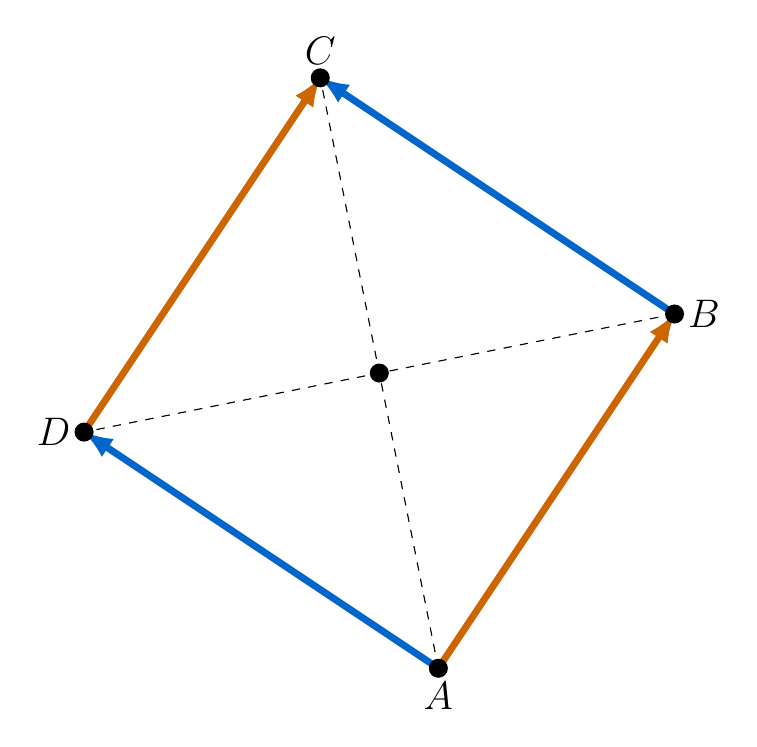
\begin{tikzpicture}[scale=1.5, font=\Large]
	\tkzDefPoint(2,3){A}
	\tkzDefPoint(4,6){B}
	\tkzDefPoint(1,8){C}
	\tkzDefPoint(-1,5){D}
	\tkzDefPoint(1.5,5.5){E}
	\draw[myblue, line width=2.5pt,-latex] (A) -- (D);
	\draw[myblue, line width=2.5pt,-latex] (B) -- (C);
	\draw[myorange, line width=2.5pt,-latex] (A) -- (B);
	\draw[myorange, line width=2.5pt,-latex] (D) -- (C);
	\draw[dashed] (A) -- (C);
	\draw[dashed] (B) -- (D);
	\node[very thick, draw, circle,fill,inner sep=2] at (A) {};
	\node[very thick, draw, circle,fill,inner sep=2] at (B) {};
	\node[very thick, draw, circle,fill,inner sep=2] at (C) {};
	\node[very thick, draw, circle,fill,inner sep=2] at (D) {};
	\node[very thick, draw, circle,fill,inner sep=2] at (E) {};
    \node[below=0.5mm] at (A){$A$};
    \node[right=0.5mm] at (B){$B$};
    \node[above=0.5mm] at (C){$C$};
    \node[left=0.5mm] at (D){$D$};
\end{tikzpicture}
\end{document}